\documentclass[a4paper,12pt]{article}
\usepackage[utf8x]{inputenc}
\usepackage{epsfig}
\usepackage{subfigure}
\usepackage{vmargin} %importante altrimenti non funziona bene la
                     %fascicolazione
\usepackage{amsmath}
\usepackage{amsfonts}
\usepackage{listings}
\usepackage{fancyhdr}
\usepackage{color}
\usepackage{url}
\usepackage{numprint}
\usepackage{placeins}
%o questo?
\usepackage{natbib}
\usepackage{multirow}

\newtheorem{theorem}{Theorem}[section]
\newtheorem{mydef}{Definition}[section]
\newtheorem{lemma}[theorem]{Lemma}
\newtheorem{proposition}[theorem]{Proposition}
\newtheorem{corollary}[theorem]{Corollary}
%\theoremstyle{plain}
\usepackage[font=small,format=hang,labelfont={sf,bf}]{caption}


%%{\wbalsup}[1] {This is the Wikibook about LaTeX supported by #1}

\newcommand{\METHOD}[1] {\textit{#1}}
\newcommand{\CLASS}[1] {\textit{#1}}
\newcommand{\nmf}{\textit{NMF}}

\lstdefinestyle{java}{
    	language=Java, 								% choose the language of the code
		basicstyle=\footnotesize,       			% the size of the fonts that are used for the code
		%numbers=left,                   			% where to put the line-numbers
		%numberstyle=\tiny,      					% the size of the fonts that are used for the line-numbers
		stepnumber=4,                   			% the step between two line-numbers. If it's 1 each line will be numbered
		numbersep=4pt,                  			% how far the line-numbers are from the code
		backgroundcolor=\color{white},  	% choose the background color. You must add \usepackage{color}
		showspaces=false,               			% show spaces adding particular underscores
		showstringspaces=false,         		% underline spaces within strings
		showtabs=false,                 				% show tabs within strings adding particular underscores
		frame=shadowbox,							% display a frame around the code
		tabsize=4,                      					% sets default tabsize to 2 spaces
		captionpos=b,                   				% sets the caption-position to bottom
		breaklines=true,                				% sets automatic line breaking
		breakatwhitespace=false,        		% sets if automatic breaks should only happen at whitespace
		escapeinside={(*@}{@*)},          		% if you want to add a comment within your code
		% added by max
		mathescape=true,					
		columns=flexible,
}

\newcommand{\javalisting}[2]{
	\lstinputlisting[style=java,label=code:#1,caption=#2]{./code/#1.java}
} 


\newcommand{\commento}[1]{\begin{color}{white}\colorbox{black}{
	\textit{\textbf{==) \texttt{ [#1] (==}}}}\end{color}
}
\setpapersize{A4}
%%\setmarginsrb{35mm}{35mm}{25mm}{35mm}{0pt}{10mm}{0pt}{5mm} %leftmargin,topmargin,rightmargin,bottom, ...
\linespread{1.25}

\lstdefinestyle{matlab}{
    	language=Matlab, 							% choose the language of the code
		basicstyle=\footnotesize,       			% the size of the fonts that are used for the code
		%numbers=left,                   			% where to put the line-numbers
		%numberstyle=\tiny,      					% the size of the fonts that are used for the line-numbers
		stepnumber=4,                   			% the step between two line-numbers. If it's 1 each line will be numbered
		numbersep=4pt,                  			% how far the line-numbers are from the code
		backgroundcolor=\color{white},  	% choose the background color. You must add \usepackage{color}
		showspaces=false,               			% show spaces adding particular underscores
		showstringspaces=false,         		% underline spaces within strings
		showtabs=false,                 				% show tabs within strings adding particular underscores
		frame=shadowbox,							% display a frame around the code
		tabsize=4,                      					% sets default tabsize to 2 spaces
		captionpos=b,                   				% sets the caption-position to bottom
		breaklines=true,                				% sets automatic line breaking
		breakatwhitespace=false,        		% sets if automatic breaks should only happen at whitespace
		escapeinside={(*@}{@*)},          		% if you want to add a comment within your code
		% added by max
		mathescape=true,					
		columns=flexible,
}

%opening
\title{Hadoop Project: Non Negative Matrix Factorization}
\author{Lottarini Andrea \\ Virgilio Daniele}

\begin{document}

\maketitle
%\tableofcontent

\begin{abstract}

The scope of this project is to implement the Non Negative Matrix Factorization algorithm with multiplicative update as presented in \citep{liu2010}.
The main application of this algorithm is for Text Mining \cite{05abstractemail}.
The algorithm is developed in a Map Reduce fashion using the Apache Hadoop framework.
We will not cover algorithmic details, but instead we will focus on the implementation of the multiplicative update method in Hadoop and study its scalability.
The Non Negative Matrix Factorization family of algorithms is presented in Section \ref{nmf} with a particular interest on the   multiplicative update method. 
A general outline of a Map Reduce implementation is presented in Section \ref{mapreduce} while implementations details are presented in Section \ref{sec:implementation}.
The final results and the outlines for future work are presented in Section \ref{result} and Section \ref{conclusion}.

\end{abstract}

\section{Non Negative Matrix Factorization}
\label{nmf}

Non Negative Matrix Factorization algorithms (NMF) are a group of numerical algorithms for matrix factorization.
A matrix A is factorized in two matrix W and H by a NMF algorithm . 
We first assume that the matrix A's elements are non negative (greater or equal by 0). 
The factorization has the property of $ A \simeq W H $ and both matrices W and H are non negative. 
This factorization is in general not unique, and in fact, let's assume that $W_1$ and $H_1$ are factors of the matrix A.
It's possible to find another factorization using a generic matrix $L$ and its inverse: $A \simeq W_1 H_1 = ( W L ) (L^{-1} H) = W_2 H_2  $. 

The non negative matrix factorization problem can be formulated as follows:
\begin{mydef} \textbf{Non Negative Matrix Factorization}
  Given a non negative matrix $A \in \mathbb{R}^{m×n}$ and a positive integer $k<min\{m,~n\} $, find non 	
  	negative matrices $W \in R^{m×k}$ and $H \in R^{k×n}$ to minimize the function  
  	$$ f ( W , H ) = \frac{1}{2} || A − W H ||_F^2$$ where $F$ is the Frobenious norm defined as
  	$|| X ||_F = ( \sum_i \sum_j( |x_{i,j}|^2 ) )^{1/2}$. 
  	\label{def:nmf}
\end{mydef}


In this way, the product of W and H is not exactly equal to A but is an approximation. 
Obviously, the smaller is the norm of the residual matrix ($D = A - WH$), the better is the approximation. 
Furthermore, by choosing a $K$ less than $\frac{m * n}{m + n} $ the space needed to store the matrix decrease.


The Non Negative Matrix Factorization (NMF) is a conical coordinate transformation \cite{Nikolaus07learningthe} where the $W$ matrix describes the basis vector and all the elements in the dataset by enclosing in the cone identified by W. 
Each element, in the cone, can be expressed as positive linear combinations of vectors in W. 
The NMF is equivalent to a relaxed form of K-means clustering where the matrix W contains cluster centroids and H contains cluster membership indicators when the least square function is used as estimator of the distance.


As previously mentioned, the non negative matrix factorization is a group of algorithms. 
The algorithm used is the Multiplicative Update Algorithm, but there exists other types of algorithms such as the Gradient Descent algorithm\cite{gradient} and Alternating Least Square Algorithm\cite{least}. 

The code of the algorithm is listed below using MatLab syntax.
\begin{lstlisting}[style=matlab,label=code:nmf,caption=Pseudocode of the multiplicative update algorithm. The .* and ./ operators stand for element by element multiplication and division.]
function [W,H] = nmf(A)

W = rand(m,k);	% initialize W as random dense matrix 
H = rand(k,n);	% initialize H as random dense matrix 

for i = 1 : number_of_iterations
	H = H .* (W' * A) ./ (W' * W * H);
	W = W .* (A * H') ./ (W * H * H');
end
\end{lstlisting}

The Multiplicative Update Algorithm generally converges to a point that is not the global minimum of $f(W,H)$ (Definition \ref{def:nmf}).
Moreover, given a pair $(W_1,H_1)$, it is also not possible to determine if $\exists \; (W_2,H_2) \; . \;f(W_2,H_2) \leq f(W_1,H_1)$, unless such a pair $(W_2,H_2)$ is found by applying the method with different initial conditions. 
Therefore, current research on the \nmf  family of algorithms focuses on how to choose initial factors in order to discover a global minimum.

More precisely, current research on Non Negative Matrix Factorization regards:
\begin{itemize}
  \item Algorithmic -- How to choose initial parameters in order to discover a global minimum instead a local minimum and speed-up the convergence process.
   \item Scalability -- How the problem can scale when the dimension of the matrix increase.
    \item Online -- How to update the factorization when new data is known without the need of a recomputing from scratch.
\end{itemize}

We will focus on the second problem.

\section{Map Reduce Algorithm }
\label{mapreduce}

For our implementation, we assumed that the distribution of the values of the input matrix was gaussian.
If this is the case, the computation has the form of Listing \ref{code:nmf}.
Now, we discuss how this rather simple algorithm can be implemented in Map Reduce\cite{liu2010}.
We will consider separately the update of the $\mathcal{H}$ matrix (Figure \ref{fig:mapReduceScheme}) and the update of the $\mathcal{W}$ matrix, even though, the two operation are very similar.

\begin{center}
	\begin{figure}[h]
	\centering
	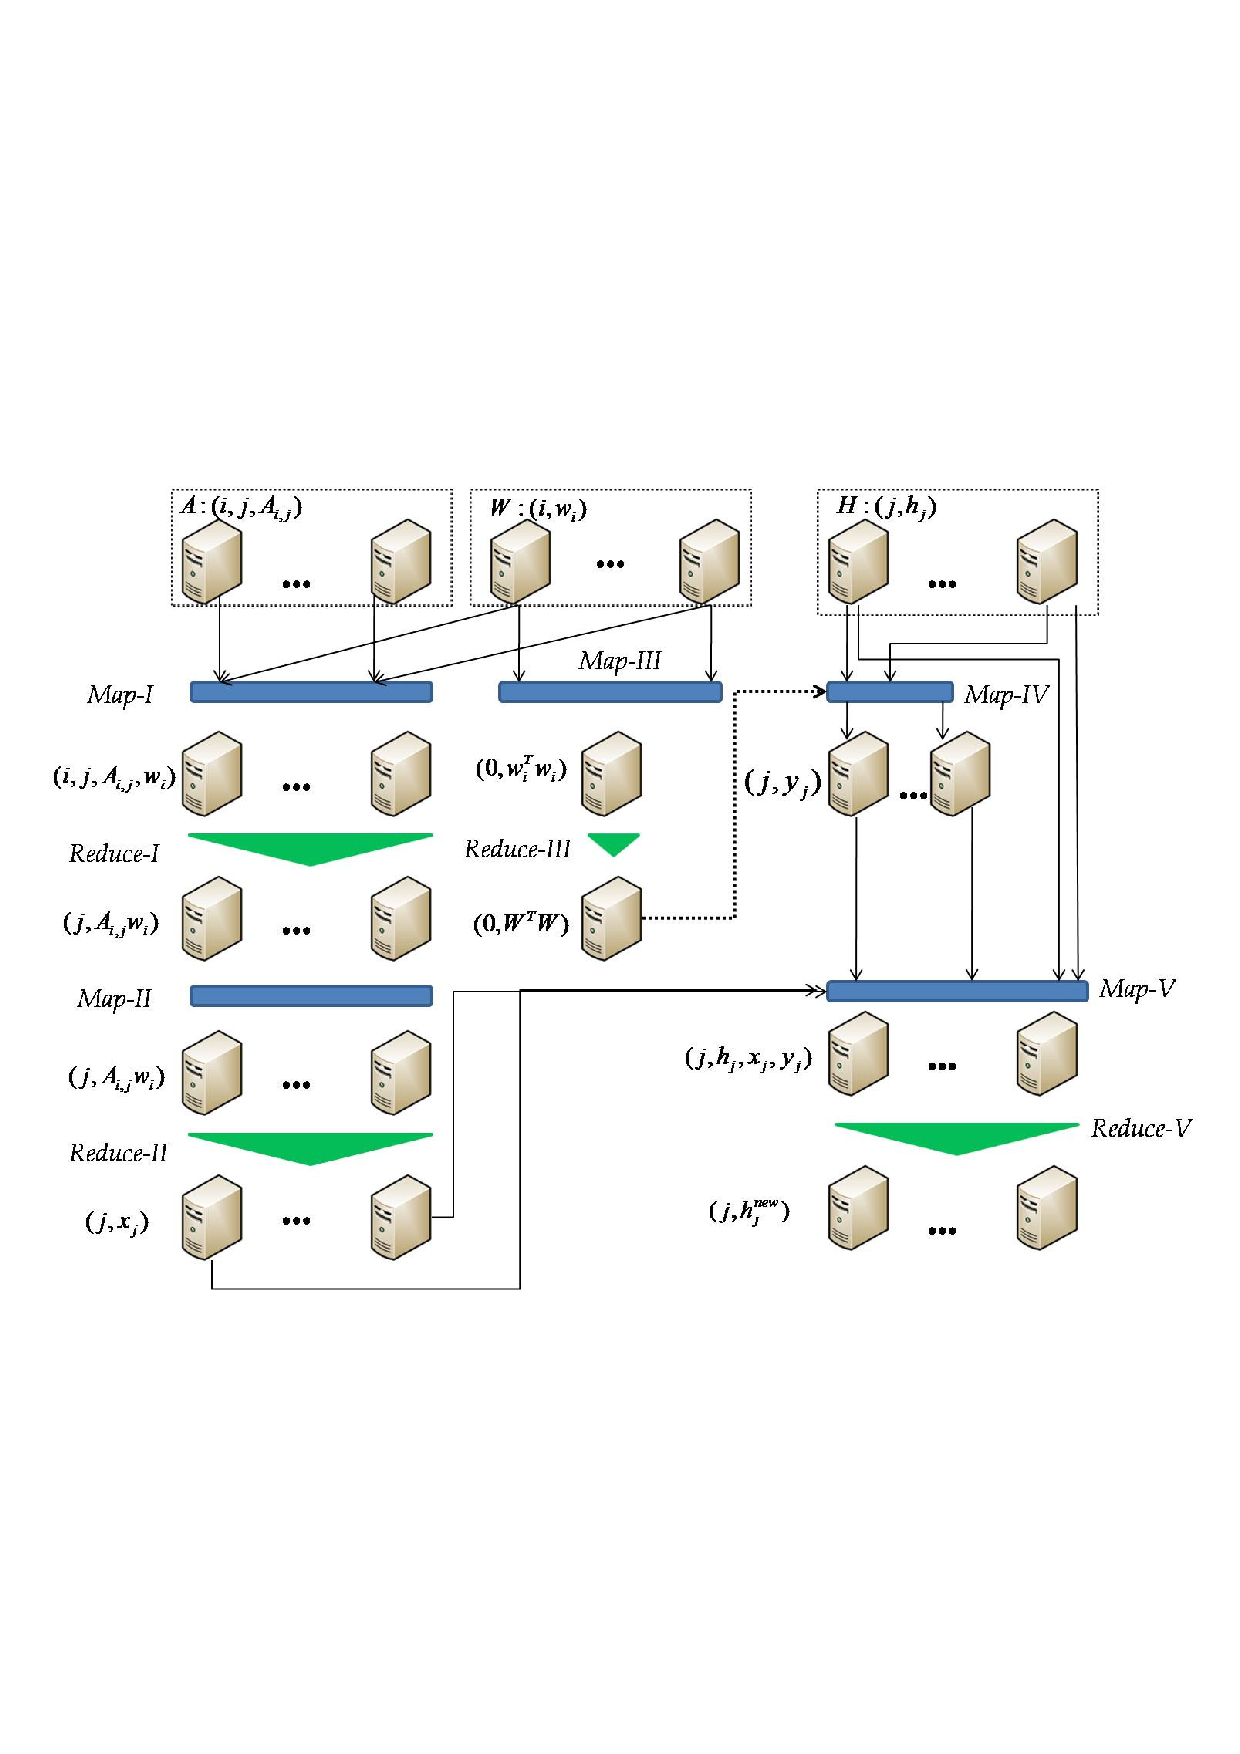
\includegraphics[width=0.9\textwidth]{./figures/mapReduceScheme}
	\caption{Update of the H matrix: $H = H.*\frac{W^T*A}{W^T*W*H}$ }
	\label{fig:mapReduceScheme}
	\end{figure}
\end{center}

 \subsection{Update of the H Matrix}
 \label{sec:hupdate}
    From Figure \ref{fig:mapReduceScheme}, we can see that the algorithm is divided in three main phases:
    
  \subsubsection{$ X = W^T * A $}
        This operation is computationally equivalent to multiplication of a sparse matrix with a vector. 
        Consider that $k$ is usually less than 100 so the matrix W is very narrow. 
		Let $x_j$ denote the $j^{th}$ column of X, and $w_i$ denote the $i^{th}$ row of W.
		We use $\mathbb{O}$ to indicate non zero elements of A, i.e. $\mathbb{O} = \{ (i,j) \;|\; A_{i,j}  \neq 0 \}$.
		Similarly $\mathbb{O}_i = \{j \;|\; A_{i,j} \neq 0 \}$ and $\mathbb{O}^j = \{i \;|\; A_{i,j} \neq 0 \}$.
		We have that
        $$ x_j = \sum_{i=1}^{m} A_{i,j} w_{i}^{T} = \sum_{i \in \mathbb{O}_i} A_{i,j} w_{i}^{T} $$ 
        This operation is implemented with two steps of map reduce.
        
        \begin{itemize}
          \item MAP-I: Map $ \langle i, j, A_{i,j} \rangle $ and $\langle i, w_i \rangle$ on i
            such that tuples with the same i are shuffled together in
            the form of  $ \langle i, \{w_{i}, (j, A_{i,j}) \forall j
            \in \mathbb{O}_i \} \rangle$.

         \item REDUCE-I: Take  $ \langle i, \{w_{i}, (j, A_{i,j}) \}
           \rangle$ and emit  $ \langle j, A_{i,j}  w_{i}^{T}
           \rangle$ $\forall j \in \mathbb{O}_i $.

          \item MAP-II: Map the $ \langle j, A_{i,j}  w_{i}^{T}
           \rangle$ on j such as tuples with the same j are shuffled
           together in the form of $ \langle j, \{A_{i,j}  w_{i}^{T} \}
           \forall i \in \mathbb{O}^j \rangle$.

          \item REDUCE-II: Take $ \langle j, \{A_{i,j}  w_{i}^{T} \}
           \forall i \in \mathbb{O}^j \rangle$, and emit $\langle j,
           x_j \rangle$ where $ x_j = \sum_{i \in \mathbb{O}^j} A_{i,j}  w_{i}^{T} $.

         \end{itemize}


     \subsubsection{$ Y = W^T * W * H $}
       It is wise to compute Y by first computing $C= W^T W$ and then
       $Y=CH$ because it maximizes the parallelism while requiring
       fewer multiplications than $Y= W^T (W H)$. 
       With the partitioning of W along the smaller dimension, calculation of $ W^T W $ can be
       fully parallelized because $$ W^T W = \sum_{i=1}^{m} w_i^T. $$
       It means that each machine can first compute $w_i^T w_i$  (a
       small k × k matrix) for all the $w_i$’s it hosts, and then send
       this partial results to a \textbf{single} reducer. 
       The C matrix must be make
       available to all the entities of the following phase as global
       shared data.

       \begin{itemize}

         \item MAP-III: Map $\langle i, w_i \rangle$ to  $\langle 0,
           w_i^T w_i \rangle$ where 0 is a dummy key value for data
           shuffling.

          \item REDUCE-III: Take $\langle 0,
           \{w_i^T w_i\}_{i=1}^{m} \rangle $ and emit $\sum_{i=1}^{m} w_i^T w_i$.

         \item MAP-IV: Map the $ \langle j, h_j \rangle$ to $ \langle
           j, y_j = Ch_j \rangle$.

       \end{itemize}


     \subsubsection{$ H = H .* X ./ Y $}
       \begin{itemize}

       \item MAP-V: Map $\langle j, h_j \rangle$, $\langle j, x_j
           \rangle$ and $\langle j, y_j \rangle$ on j such that tuples
           with the same j are shuffled together in the form of
           $\langle j, \{h_j, x_j, y_j\} \rangle$.

         \item REDUCE-V: Take $\langle j, \{h_j, x_j, y_j\} \rangle$
            and emit $\langle j, h_j^{new} \rangle$ where $h_j^{new} =
            h_j .* x_j ./ y_j $.

          \end{itemize}

	
	\subsection{Computation of the updated W Matrix}
    This sequence of phases is very similar to the update of the H matrix.

    \begin{itemize}
      \item \subsubsection{$ X = A * H^T $}
        This phase is computationally equivalent to a matrix vector multiplication. The only difference with phase 1 of the update of matrix H is the fact that in this case the order of multiplication of the matrix and the vector is reversed. 
        Let $x_i$ denote the $i^{th}$ row of X, then 
        $$ x_i = \sum_{j=1}^{m} A_{i,j} h_{j} = \sum_{j \in \mathbb{O}_i} A_{i,j} h_{j} $$
        This operation is implemented as two set of map/reduce
        operations.
        \begin{itemize}
          \item MAP-I: Map $ \langle i, j, A_{i,j} \rangle $ and $\langle j, h_j \rangle$ on j
            such that tuples with the same i are shuffled together in
            the form of  $ \langle j, \{h_{j}, (i, A_{i,j}) \forall i \in \mathbb{O}_j \} \rangle$.

         \item REDUCE-I: Take  $ \langle j, \{h_{j}, (i, A_{i,j}) \}
           \rangle$ and emit  $ \langle i, A_{i,j}  h_{j} \rangle$ $\forall i \in \mathbb{O}_j $.

          \item MAP-II: Map the $ \langle i, A_{i,j}  h_{j} \rangle$ on i such as tuples with the 
            same i are shuffled together in the form of $ \langle i, \{A_{i,j}  h_{j} \}
           \forall j \in \mathbb{O}_i \rangle$.

          \item REDUCE-II: Take $ \langle i, \{A_{i,j}  h_{j} \}
           \forall j \in \mathbb{O}_i \rangle$, and emit $\langle i,
           x_i \rangle$ where $ x_i = \sum_{j \in \mathbb{O}^i} A_{i,j}  h_{j} $.

         \end{itemize}

     \item \subsubsection{$ Y = W * H * H^T $}
       It is wise to compute Y by first computing $C= H H^T$ and then
       $Y=WC$. 
       The C matrix must be made available to all the entities
       of the following phase as global
       shared data.

       \begin{itemize}

         \item MAP-III: Map $\langle j, h_j \rangle$ to  $\langle 0,
           h_j h_j^T \rangle$ where 0 is a dummy key value for data
           shuffling.

          \item REDUCE-III: Take $\langle 0, \{h_j h_j^T\}_{j=1}^{n}
            \rangle $ and emit $\sum_{j=1}^{n} h_j h_j^T $.

         \item MAP-IV: Map the $ \langle i, w_i \rangle$ to $ \langle
           i, y_i = w_iC \rangle$.

       \end{itemize}


      \item \subsubsection{$ W = W .* X ./ Y $}
        \begin{itemize}

         \item MAP-V: Map $\langle i, w_i \rangle$, $\langle i, x_i
           \rangle$ and $\langle i, y_i \rangle$ on i such that tuples
           with the same j are shuffled together in the form of
           $\langle i, \{w_i, x_i, y_i\} \rangle$.

          \item REDUCE-V: Take $\langle i, \{w_i, x_i, y_i\} \rangle$
            and emit $\langle i, w_i^{new} \rangle$ where $w_i^{new} =
            w_i .* x_i ./ y_i $.

       \end{itemize}

    \end{itemize}

\section{Implementation}
\label{sec:implementation}

In this section we will analyze the implementation choices and specify the Hadoop's key features that were used. 
We refined our implementation many times as we became more confident with the framework and its mechanism: every modification leading to better performance and more maintainable code.
We are going to first introduce the motivations that guided our design choices and some of the \textit{breakthrough} on the framework that made us restart from scratch.
Then, we will comment in detail on the implementation of the various phases.

\paragraph{Types}
Our first implementation used mainly Text as key or value type.
This is convenient since the programmer has complete control on how information is passed from one stage to another.
It is also very easy to build an application storing all information as text.
However, this solution had some problems:
\begin{itemize}
\item Code is not easily \textbf{maintainable} and \textbf{modifiable} as every phase performs string manipulation. 
Making a modification on the pattern of storage of information requires modification in all the codebase.
\item Storing matrices as text pose problems of space occupancy, precision and efficiency. 
In fact, storing floating point values as text is inefficient in terms of space.
Moreover, in order to perform arithmetic operations it is necessary to parse numeric values, perform the operation and convert them back to string.
This leads to poor performance and excessive garbage collection.
\end{itemize}
Therefore, we decided to create our types of data that can be transmitted as key or value type.

In order to achieve this goal, each classes representing an object in our application implements the interface \CLASS{WritableComparable} of the Hadoop framework and overrides the methods:
\begin{itemize}
  \item \METHOD{ReadFields()} / \METHOD{WriteFields()} - for reading/writing the data in a serializated format.
  \item \METHOD{compareTo()} - for comparing two element in the case the type is used as key.
\end{itemize}

Also, dual methods for reading and writing in human-readable format is defined in the method \METHOD{parseLine()} and \METHOD{toString()}.
The mathematical operations that can be done on the different types are implemented directly in the class as instance method (e.g. multiplication matrix per vector, vector per vector and so on).

We implemented the following classes:
\begin{enumerate}
  \item NMFVector: Vector datatype with associated numerical operations. 
  \item NMFMatrix: Matrix datatype with associated numerical operations.
  \item SparseElement: Element of a Sparse Matrix.
  \item SparseVectorElement: Element with a single coordinate.
  \item IndAndIdWritable: A particular datatype used in the first phase and last phase.
\end{enumerate}

IntAndIdWritable will be explained in detail in Section \ref{sec:phase1}.
The other types are quite self explanatory, but NMFVector requires a few words.
Every vector from matrix W and H has a fixed length $k$; it is inefficient to serialize the length information for every element.
Therefore, we did not use \textit{ArrayWritable}, but defined our own datatype.
The length of vectors is stored as a static attribute of the NMFVector class and initialized in every mapper and reducer using a context variable.
The context variable is initialized in the main of every phase.

These classes can be used as intermediate keys or values; however, we want that each phase uses our datatypes as input and output elements.
This is possible using \textbf{Sequence Files.}

\paragraph{Sequence Files}

Hadoop also offers the possibility to use as Input and Output of a map reduce job serialized data (binary data). 
This is done via the SequenceFile record reader and writer.
This mechanism also produces a more readable and efficient code since the key value pairs are stored as objects, instead of Text, which eliminates the need for conversion.
Different tools (written as of Map/Reduce programs) for converting the data from text to binary and vice-versa were also implemented.

\paragraph{Data Flow}

We wanted to keep every phase (Figure \ref{fig:mapReduceScheme}) separated in order to ease debugging and performance tests.
However, update of the W and H matrix are complex operation that requires 5 steps each.
Therefore, we developed a set of bash scripts to control input and output folder and maintain a consistent state on the distributed file system.
This is very important since folder names should be chosen wisely in order to ensure correctness of the application (see Section \ref{sec:phase1} and \ref{sec:phase5})

\paragraph{Optimization of communications and object creation}

It is very important to try to reduce the amount of data transferred in order to ensure maximum performance.
Therefore, we used combiners in every phase that could benefit from them.
We also tried to reduce the amount of objects created in each phase in order to reduce garbage collection.
Moreover, we implemented phase 1 with particular attention in order to maintain a streaming model of computation,  (Section \ref{sec:secondary}).

Specific implementation details on each phase can be found in the following sections.

\subsection{Phase 1}
\label{sec:phase1}

This phase is both the most complex to implement and the most greedy in terms of resources.
Therefore, we tried to implement it in the most efficient way.
We had to change our design multiple times so we are going to thoroughly explain the optimizations that we used.

We already explained in Section \ref{sec:hupdate} that the first and second phase correspond to a matrix vector multiplication since the W matrix is very narrow.

\begin{center}
	\begin{figure}[h]
	\centering
	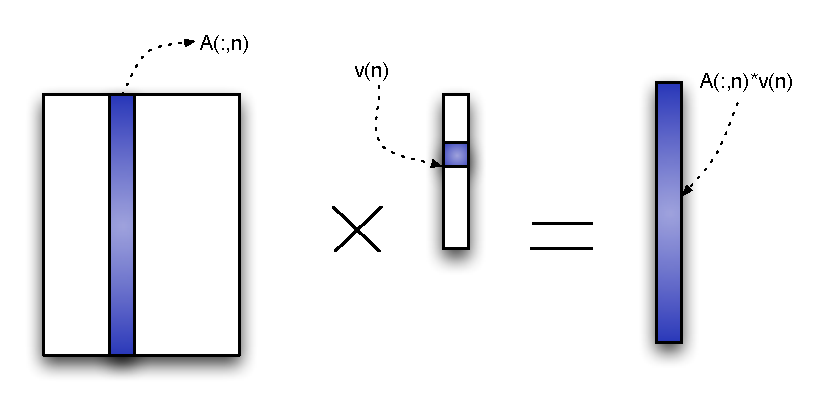
\includegraphics[width=0.9\textwidth]{./figures/Map1}
	\caption{First Phase of Map Reduce}
	\label{fig:Map1}
	\end{figure}
\end{center}

It does not appear to be a complex operation to implement in Hadoop, but it requires some attention in order to be implemented correctly.
The first step in particular is somewhat tricky. 
Let's analyze it in detail.
\begin{enumerate}
\item The mapper should distinguish between the elements of matrix A and the vector elements of matrix W. 
It also has to emit data structured differently in the two cases.
\item Similarly, the reducer has to distinguish between the elements  of matrix A and the vector elements of matrix W.
\item Consider the output of the reducer $ x_j = \sum_{i=1}^{m} A_{i,j} w_{i}^{T} = \sum_{i \in \mathbb{O}_i} A_{i,j} w_{i}^{T}$.
 We would like to receive vector $w_i$ before the elements of the matrix since $w_i$ is used in every multiplication performed by the reducer.
\item We are using two steps of map reduce in sequence and the information is not implicitly text (they are numbers) and we would like to minimize the size of the data transferred.
\item We want to have a well organized/maintainable code.
\end{enumerate}

\FloatBarrier
The first two concerns are functional, in fact it is necessary to distinguish elements from A and W, otherwise the computation will be incorrect.
First we consider a preliminary straightforward implementation (Listing \ref{code:Map1Text}).

We solved the problem of distinguishing between A and W in the mapper using the filename of the chunk. 
Similarly, we solved the problem in the reducer by adding an annotation in the intermediate values. 
Now, Mappers and Reducers can distinguish between data from the two matrices.
We are also using text to save intermediate values so we can arrange the structure of the data as we want.
Now, we consider non functional constrains.
This solution is inefficient since the reducer has to store every element received from the matrix. 
The order of the values received is random.
A possible optimization is to buffer elements from A \textbf{until} the element from the vector is received and then, flush the buffer and output final elements in a streaming fashion.
In the worst case, this solution is equivalent to the previous solution (Listing \ref{code:Map1Text}).
We can overcome this problem using the shuffle \& sort phase and ensure that the vector element will be the first on the list of values for every reduce operation.
This problem of having values (not only keys) sorted can be found in literature as \textbf{Secondary Sort}.

\subsubsection{Secondary Sort}
\label{sec:secondary}


What we want to accomplish with secondary sort is to have runs of values from a key ordered depending on our needs.
There are many possible ways to implement a secondary sort; in this case a very convenient solution is to define a specific object as a key.
In order to utilize a user defined object as a key in Hadoop, it must implements the WritableComparable interface.
The object must be comparable so that a list of keys can be sorted using their compareTo method. 
The object must be writable in order to be serialized using the methods readFields(DataOutput out) and write(DataInput in). 
In this specific case, we can extend IntWritable (Listing \ref{code:IntAndIdWritable}) in order to solve the problem in a very concise way.

Consider the three phases that occur during shuffle \& sort.
\begin{enumerate}
\item Sort: elements are sorted. Based exclusively on the key.
\item Partition: elements are partitioned to worker, this is based both on the key and the value (if necessary).
\item Group: elements are grouped together in a single reduce() invocation. 
The user can override the comparator and group together elements with different keys. Notice that every object can have different comparators for the sort and group phase.
\end{enumerate}

The first phase sorts the output from the mappers using the key. 
In our class, we added an id and implemented a new compareTo method so that elements will be in the right order (element from the vector first).
To be more efficient, the framework gives the programmer the possibility to implement a compare directly on the bytes of the serialized object in order to avoid serialization and deserialization during the shuffle \& sort phase.
The inner class Comparator implements such compare on bytes.
By doing so, the Sort phase will place the element coming from the vector \textbf{before} the elements from the matrix.
However, this is not enough because elements from the vector and the matrix have different keys so they could be partitioned to different machines.
We must ensure that they are sent to the same reducer task.
This is done by defining an ad hoc partition function which in this \textbf{particular} case can be inherited from the superclass (IntWritable) without any modification. 
The IntAndIdWritable class will inherit the hashcode method from the IntWritable class and the default HashPartitioner will be used.
Therefore, only the integer part of the object will be used for partitioning.
By doing so, runs of elements will be assigned to the same reducer without considering the id, i.e. without considering if they are elements from the matrix or from the vector.
Still this is not enough. 
We ensured that the elements from the matrix and the vector having the same index are sent to the same reducer and they are sorted in such a way that the element from the vector is the first of the run. 
Now, we would like to receive both on a single sorted run invoking reduce().
This is done by implementing a grouping comparator; a grouping comparator tells the framework when to collapse different runs (with different keys) in a single run. 
In this specific case, we can declare the comparator of IntWritable as grouping comparator of IntAndIdWritable so elements with the same integer part will be grouped together ignoring the id.

The whole implementation of secondary sort is not so simple since it requires redefinition of the different mechanisms.
In this case, we managed to implement it with minimal modifications using the default partitioner and inheriting other mechanisms from IntWritable. 
The reader may actually benefit from trying to implement the Secondary Sort from scratch redefining all the three interfaces (all the methods should work on raw binary data for better performance).

\subsubsection{Generic Objects and Sequence Files}

Now, consider a completely different problem of the naive implementation (Listing \ref{code:Map1Text}): we work with integers and double values and therefore using text for input/output and intermediate values is probably inefficient and leads to complex code.
For intermediate values, Hadoop offers the possibility to use any type under the constrains that it should implement the WritableComparable interface.
Hadoop also offers the possibility to use as Input and Output of a map reduce job serialized data (binary data). 
This is done via the SequenceFile record reader and writer.
This mechanism also produces a more readable and efficient code since key value pairs are stored as objects, instead of Text, without need for conversion. 
In our case, the input key will correspond to the column index of either the matrix or the vector.
Similarly to what presented in Listing \ref{code:Map1Text}, we can distinguish vector or matrix element from the filename.

However, we have the problem that values read from the input and emitted from mappers can either be a sparse element (value and coordinates) or a double value (a single vector element).
Consider that it is not possible to exploit polymorphism; every object read or written by mappers and reducers must have the same \textbf{exact} type as specified in its type declaration\footnote{Consider a $Mapper<IntWritable,DoubleWritable,IntWritable,DoubleWritable>$. It should be possible to read an IntAndIdWritable (which inherit from IntWritable) as a key. Similarly it should be possible to write an IntAndIdWritable as an output key. However the framework does not permit such operations.}.
Even if this breaks the Liskov substitution principle (which can be quite shocking for some of the readers of this report ), it is done in order to ensure better performance.
In fact, in order to use polymorphism, every serialized element should contain a serialized id of its class increasing the amount of data transferred.
This is done in the implementation of ObjectOutputStream in Java and it greatly increases the dimension of serialized data.
Consider that in most cases, we do not want to serialize every possible type of object, but only a small set of different types.
The framework has a specific solution to solve this problem: the GenericWritable Interface. 
It provides the developer with a writable wrapper for different types of objects with a minimum overhead for serialization.

In conclusion, Secondary Sort, Sequence Files and GenericWritable elements are used in order to ensure maximum performance and produce a concise and maintainable code.
The final implementation is presented in Listing (\ref{code:HPhase1}):
 
Notice how objects are reused in order to reduce the overhead of garbage collection and this overhead might be significant for very large computations (especially if jvm reuse is enabled).

The final implementation of the phase 1 has the following structure:

        \begin{itemize}
        
          \item MAP: Read from the input either SparseElements from Matrix A  or  row vectors of matrix W.
          \begin{itemize}
          
          \item SparseElements: Read pairs $\langle i,( j, A_{i,j}) \rangle $ of type \\
          $<$IntWritable , GenericWritable(SparseVectorElement)$>$.
          \\
          Emits pairs $\langle (i,"A"),( j, A_{i,j}) \rangle $ of type \\ 
          $<$IntAndIdWritable , GenericWritable(SparseVectorElement)$>$.
          
          \item Vector: Read pairs $\langle i, w_i \rangle$ of type \\
          $<$IntWritable , GenericWritable(NMFVector)$>$.
          Emit pairs $\langle (i,"W"), w_i \rangle$ of type \\
          $<$IntAndIdWritable , GenericWritable(NMFVector)$>$.          
          \end{itemize}

		\item SHUFFLE \& SORT: Elements from the same index are grouped together.
		Using secondary sort elements are sorted in the following order: $$\langle (i,"W"), w_i \rangle,\langle (i,"A"),( j_1, A_{i,j}) \rangle , \langle (i,"A"),( j_2, A_{i,j}) \rangle , \cdots$$ where $j_1,j_2,\cdots \in \mathbb{O}_i $.
			
         \item REDUCE: Take  $ \langle i, \{w_{i}, (j, A_{i,j}) \}
           \rangle$ and emit  $ \langle j, A_{i,j}  w_{i}^{T}
           \rangle$ $\forall j \in \mathbb{O}_i $.

         \end{itemize}

%\javalisting{HPhase2}{Second phase of matrix vector multiplication (Figure \ref{fig:Map2}). Only the Reducer is shown since non computation is performed in the Map phase.}

\subsection{Phase 2}
\label{sec:phase2}

The second phase of the $W^T*A$ operation is very simple compared to the first one.
Vectors from the first phase are grouped together using the column index, summed, and final column vectors of the matrix X are emitted (Figure \ref{fig:Map2}).
The computation is composed by:
\begin{itemize}
          \item MAP: Is the identity mapper.
			\item COMBINER: Receive vectors from local mappers sharing the same column index and periodically output partial sums.
          \item REDUCE: Receive partial vector sums from combiners as $<$IntWritable columnIndex, NMFVector values$>$. 
          Runs of values will contain all vectors having the same column index $j$. 
          Emit $\langle j, x_j \rangle$ where $ x_j = \sum_{i \in \mathbb{O}^j} A_{i,j}  w_{i}^{T} $ as a $<$IntWritable , GenericElement$>$ pair.
\end{itemize}
This phase can greatly benefit from a combiner (in fact we implemented an ad hoc combiner for this phase).
We could have used the Reducer as a combiner but notice that the Reducer has to change the type of values from NMFVector, to GenericElement, since matrix X is used as input of phase 5.
Performance gain relative to the combiner is shown in Table \ref{comb_table}.

\begin{center}
	\begin{figure}[h]
	\centering
	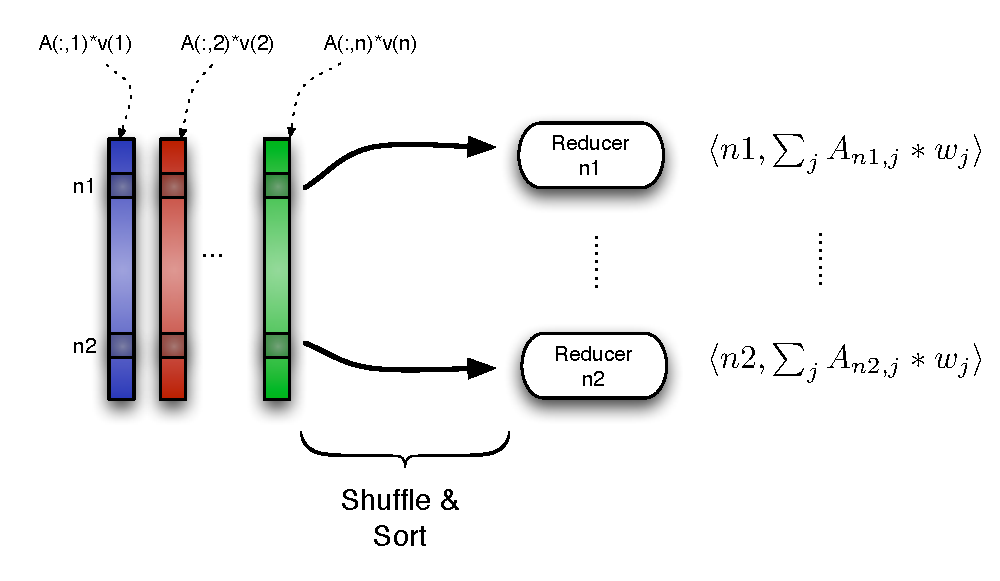
\includegraphics[width=0.9\textwidth]{./figures/Map2}
	\caption{Second Phase of Map Reduce}
	\label{fig:Map2}
	\end{figure}
\end{center}

\subsection{Phase 3}
\label{sec:phase3}

This phase performs a matrix matrix multiplication, $C=W^T*W$.
Notice that $C \in \mathbb{R}^{k*k}$ so it is very small compared to $W$.
Therefore, this operation can be computed efficiently with just one step of Map Reduce.

       \begin{itemize}

         \item MAP: Read from Input pairs of type $<$IntWritable,NMFVector$>$ containing $\langle i, w_i \rangle$ and emit pairs of type $<$NullWritable,NMFMatrix$>$ containing  $\langle -,w_i^T w_i \rangle$.

          \item REDUCE: Since NullWritable is used in the Map Phase, a single Reducer will be instantiated. It will receive a single run of values of type NMFMatrix to be summed ($\langle 0,\{w_i^T w_i\}_{i=1}^{m} \rangle $). It will emit the final result $\sum_{i=1}^{m} w_i^T w_i$ as a pair $<$NullWritable,NMFMatrix$>$.

       \end{itemize}
Notice how we used NullWritable both to reduce communications (we could have used a dummy key) and to send all intermediate values to a single reducer.
It could seem that this phase could be a bottleneck for the whole application since the reduce phase is performed sequentially on a single node.
However, by using combiners, we can solve this problem.
The Reducer will receive partial sums of the set of matrices $\langle 0,\{w_i^T w_i\}_{i=1}^{m} \rangle $.
A comparison of the number of records with or without combiner is shown in Table \ref{comb_table}.

\subsection{Phase 4}
\label{sec:phase4}

This phase is another matrix multiplication; also in this case we can implement it efficiently just using a Map phase.
This is possible since the matrix C produced in the previous step is very small.
Therefore, every node can access it and store it in local memory very efficiently.

\begin{itemize}

         \item MAP: In the setup phase, it stores in a local buffer the Matrix C.
         			Then, it reads from input the pairs $ \langle j, h_j \rangle$ of type $<$IntWritable, NMFVector $>$ and produce $ \langle j, y_j = C*h_j \rangle$.

\end{itemize}

Notice that the matrix C cannot be passed as a standard input of Hadoop.
Instead, the file must be read directly from the Distributed File System by every mapper during the setup phase. 
In our project, we assumed that the user provides, through the command line the path where the C matrix is stored. 
Using the \CLASS{FileSystem} class, it is possible to access the desired file while the file content can be read using an instance of \CLASS{SequenceReader}.

\subsection{Phase 5}
\label{sec:phase5}

Phase 5 performs the following operation:
$$ H = H.*X./Y$$
This is a \textbf{pointwise} operation so it could be performed in a single Map Reduce step very efficiently.
In fact, every column of $H_{new}$ could be computed independently of the other.
\begin{itemize}

         \item MAP: Read vectors of data from either matrix H,X or Y as pairs of type $<$IntWritable , GenericElement$>$.
         As usual, the key is the index of the vector in the Matrix.
         It emits the pairs as $<$IntAndIdWritable , GenericElement$>$ so $\langle j, h_j \rangle$ becomes $\langle (j,h), h_j \rangle$.

          \item REDUCE: Every Reducer receives three pairs: $\langle (j,h), h_j \rangle$, $\langle (j,x), x_j \rangle$ and $\langle (j,y), y_j \rangle$. They are received in this exact order since secondary sort is used. It emits $<j,h_{new}> = \langle j, h_j*x_j/y_j \rangle$.

\end{itemize}

This phase is quite straightforward.
Notice that we used secondary sort in order to receive vectors from X,H and Y in a predefined order and simplify the reducer phase.

\subsection{Update of the W matrix}
\label{sec:Wphase}

There are few differences between update of the H and the W matrix.
In fact, only phase 1 and 4 contain small modifications in the code with respect to the update of the H matrix.
These are the differences:
\begin{enumerate}
\item Phase 1: Matrix W and H are stored as $<row, (column,value)>$. 
The Mapper has to invert the order between row and column index producing $<(column,id),(row,value)>$.
\item Phase 4: The matrix C is read during the setup phase as in \ref{sec:phase4}. 
However, we have to perform $W*C$ instead of $C*Y$.
Therefore, a \textbf{left} matrix vector multiplication method is used.
\end{enumerate}

We could have collapsed these small differences between the W and H matrix update.
However, we wanted to maintain code as simple (and fast) as possible even if it leads to some duplication of code.

\section{Result}
\label{result}

To compare the results shown in the article \cite{liu2010}, we test our implementation for all reported cases in the article. All the tests reported below are executed on Pianosa\footnote{Pianosa web site: \url{http://pianosa.di.unipi.it/Home_pianosa/html/info.html}}, the Computer Science Department's Cluster in Pisa. The cluster is composed by 24 homogeneous nodes. The nodes are 800 Mz Pentium III with 1GB of main memory and they are connected together through a Fast Ethernet interconnection network. On that cluster, we installed an Apache Hadoop 0.20.2 framework. The configuration parameters are set to default, so, the maximum number of task per node is set to 2 and the number of replication is set to 3. In our configuration, we decide to place the secondary node and the job tracker in cluster interface node that is not used also as task tracker. Only other 21 nodes are available as slave, cause to momentarily unavailability of the other nodes.

The data used in the test are generated by two matrix generators written in Matlab: one for the matrix A and other one for the matrices W and H. Both generators produce positive elements Gaussian distributed. The first one is a sparse matrix generator and its sparsity factor can be tuned through an input parameter. The second one, instead, is a complete matrix generator. For our tests, we fix the $m$ and $n$ parameters (the dimension of the A matrix) respectively to $105000$ and $20000$.

For all the test we did, the reduce task number is set to $ 1,8 * number\_of\_worker$, except in the phase 3 and 4 that have a fixed number of reduce tasks. This choice has been driven by the Hadoop User Guide that suggest to set the reduce task number to $$ mapred.map\_reduceMaximumTask * number\_of\_worker * C $$ where C is a constant choose in the range $[ 0.9, 1.8]$. For a value chosen in that range, it claim that the number of reduce tasks is optimal. In our experiments, we set that constant C to 0.9. Also for the first  W/H update, the input file number can be set in the proper way. In fact, the External Phase classes (that convert the input data from text to sequence) allow to specify how many reducer tasks must be used. In that way, an equal number of file are produced.

The first test battery done tests how the computation scales in relation to the the size of the data submitted. So, we study how the performances change varying the sparsity factor of the A matrix and setting different k values. In the first test, the number of non-zero elements in the sparse matrix has been changed between $5000000$ and $80000000$ elements while the k parameter remain fixed to 10. In the second one, instead, the k value has been varied between 10 and 125 while the non zero element of the A matrix has been fixed to $16500000$.  Both tests have been executed with 16 slave nodes for three iterative updates. The mean completion time of one iterative W/H update is reported in the figure \ref{DeltaVar}  and \ref{kVar}. 


\begin{figure}[th]
	\centerline{
		\mbox{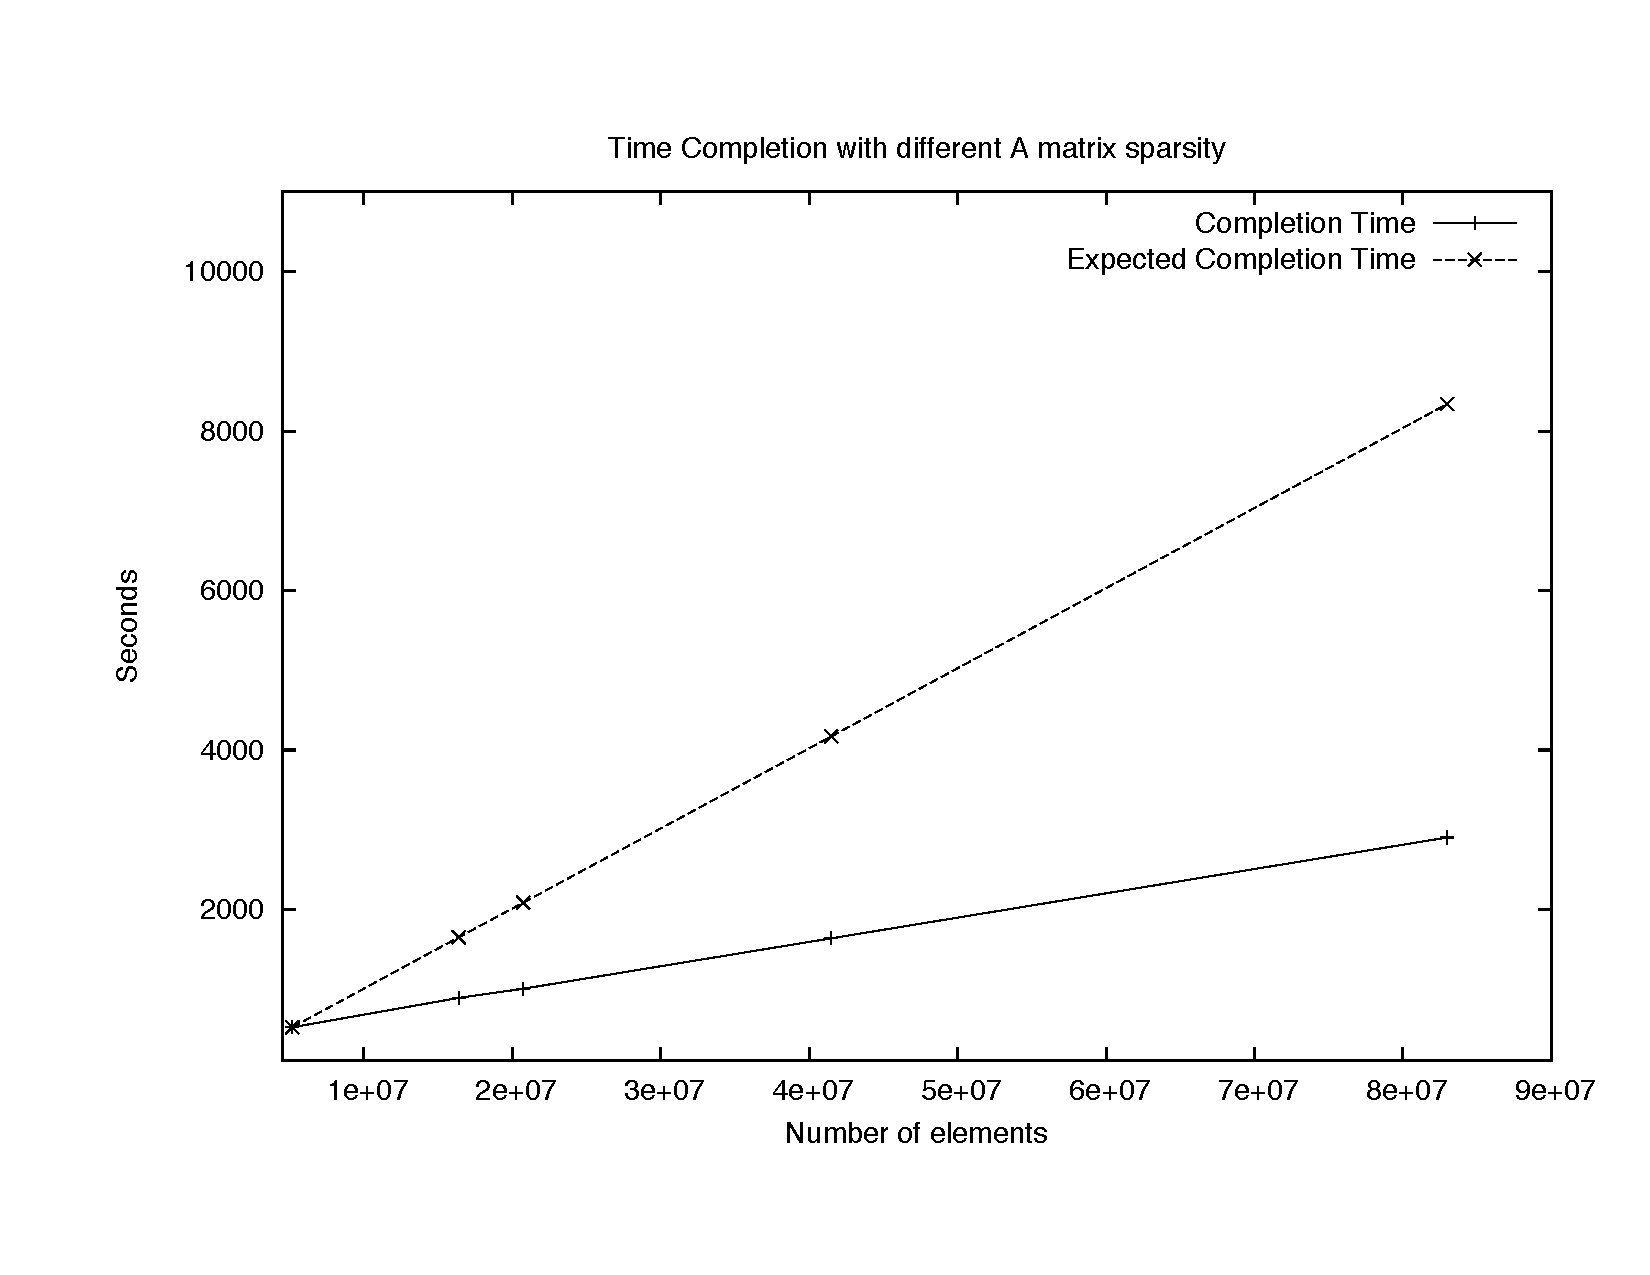
\includegraphics[scale=0.48]{HadoopTest/PsFiles/DeltaVar.pdf}}
	}
	\caption{Time Completion with different A matrix sparsity} 
        \label{DeltaVar}
\end{figure}

\begin{figure}[th]
	\centerline{
		\mbox{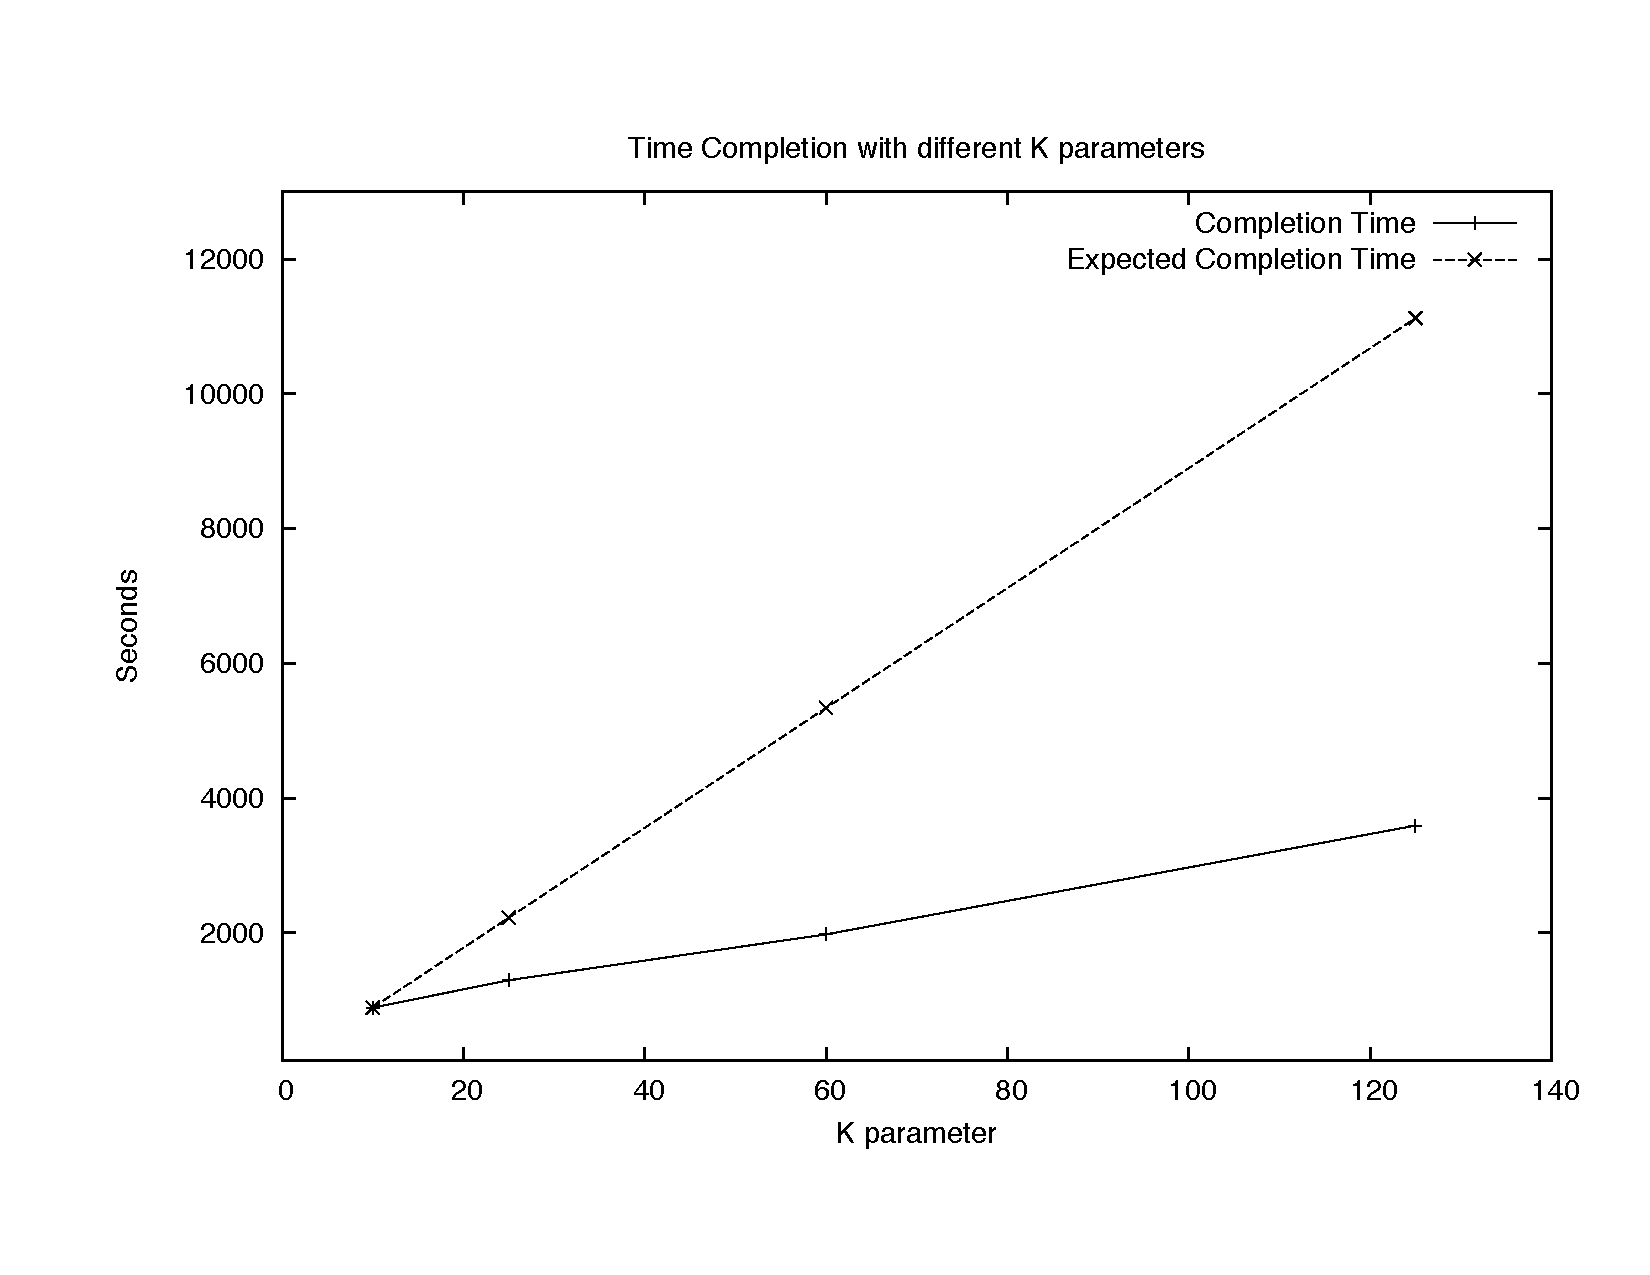
\includegraphics[scale=0.48]{HadoopTest/PsFiles/kVar.pdf}}
	}
	\caption{Time Completion with different K parameters} 
        \label{kVar}
\end{figure}


As we can see from both graphs, the behaviour of the test show a sub-linear dependencies from the size of the input data. \\

The second test battery points to examine the behaviour of the implementation when the parallel degree of the computation vary in the range $[1, 21]$. The results of the test are reported in the figure \ref{NTime}  and \ref{NScal}. The first graph focuses the attention on the completion time while the second one on the scalability.


\begin{figure}[th]
	\centerline{
		\mbox{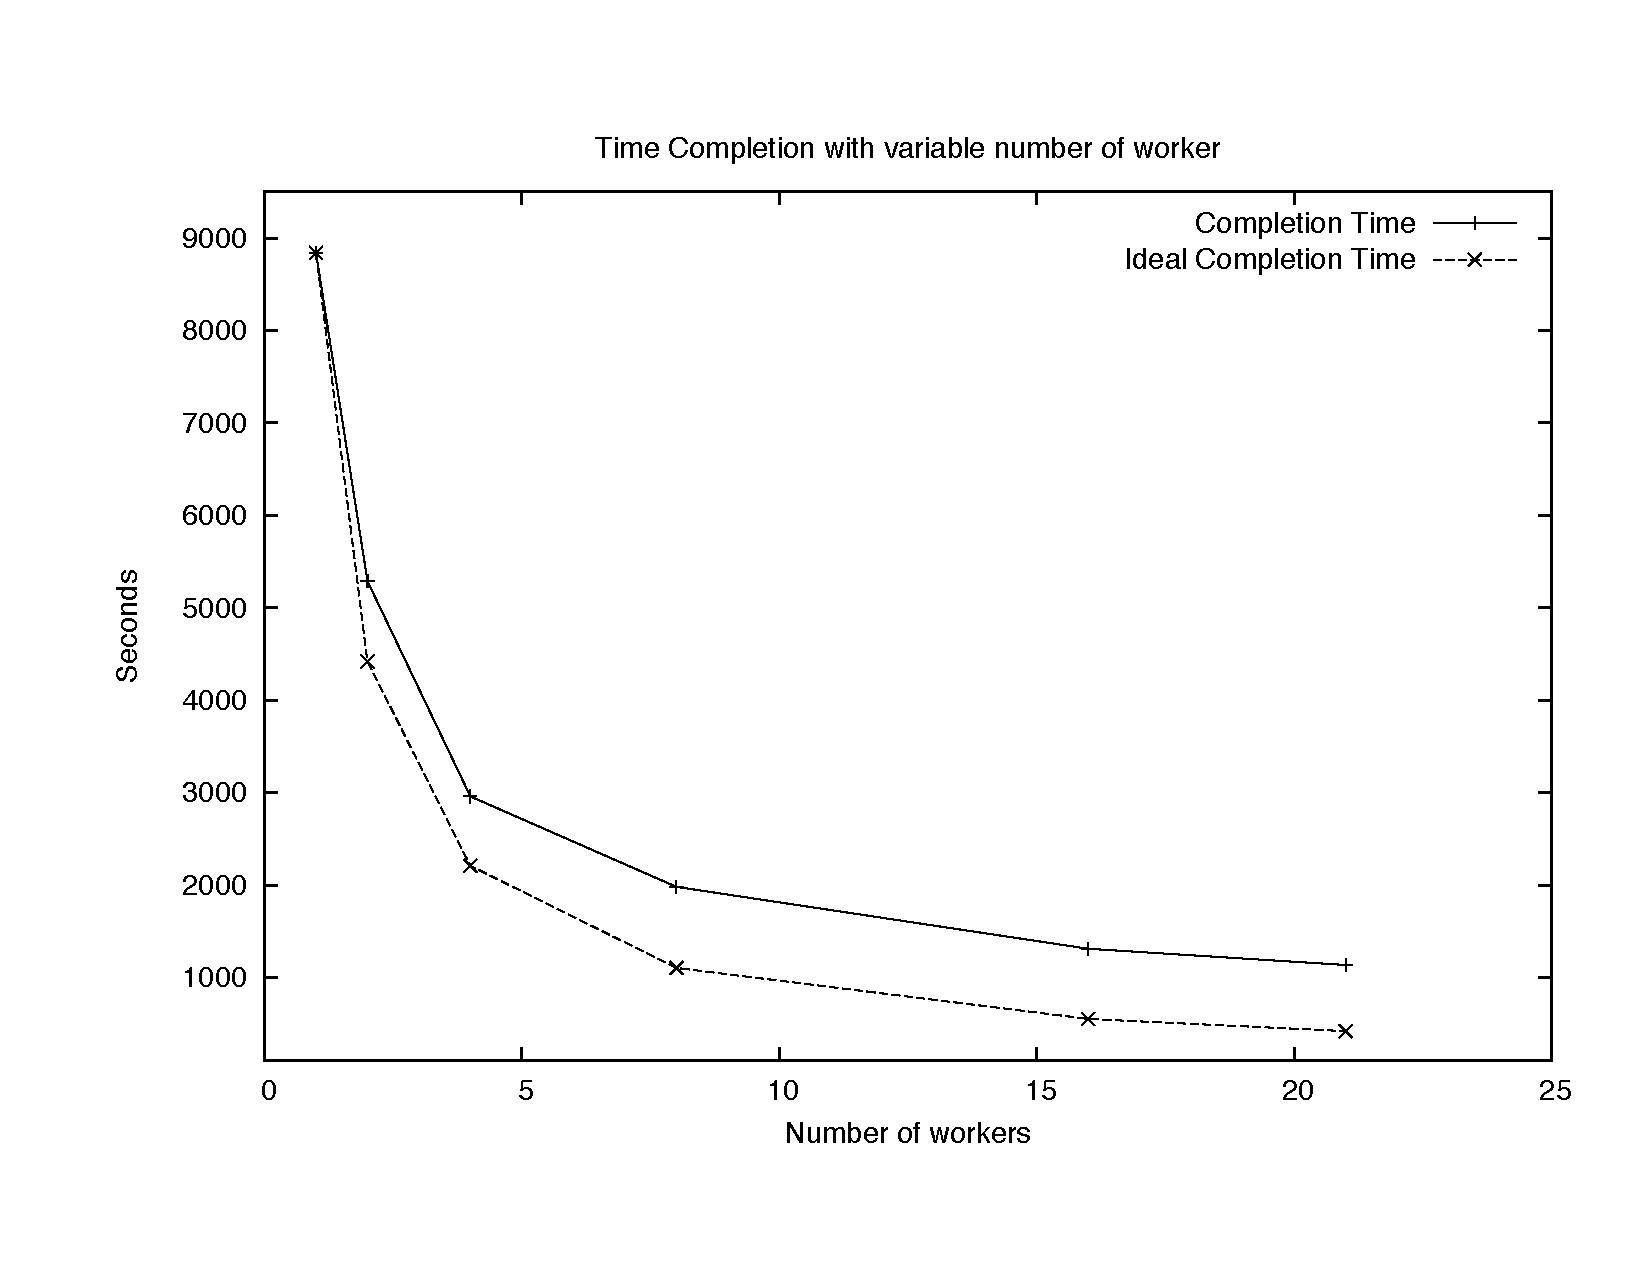
\includegraphics[scale=0.48]{HadoopTest/PsFiles/NTime.pdf}}
	}
	\caption{Time Completion with variable number of worker} 
        \label{NTime}
\end{figure}

\begin{figure}[th]
	\centerline{
		\mbox{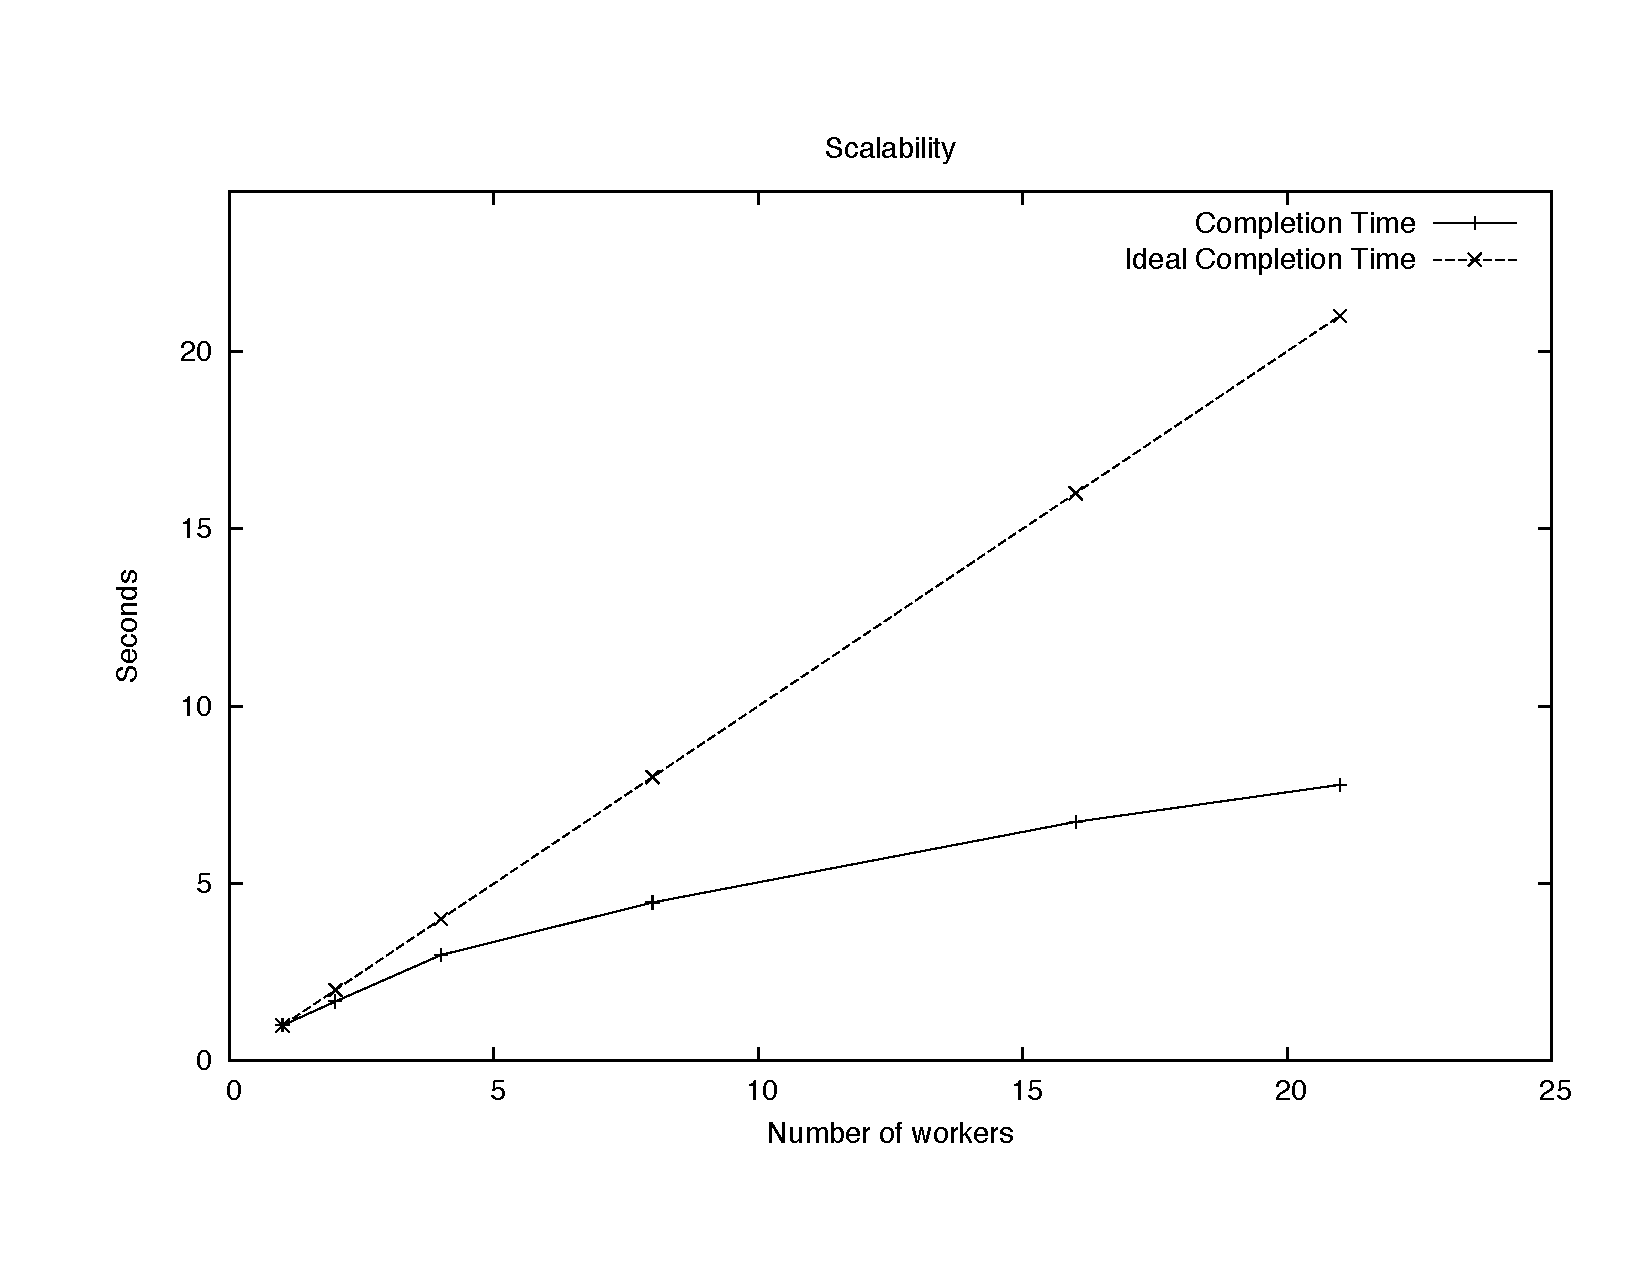
\includegraphics[scale=0.48]{HadoopTest/PsFiles/NScal.pdf}}
	}
	\caption{Scalability} 
        \label{NScal}
\end{figure}

As we can see from the figure \ref{NScal}, the implemented algorithm doesn't scale vary well. This is due mainly to two different facts: some phases in the computation doesn't scale adding more slave nodes and other phases, instead, doesn't exhibit an optimal scalability. An example of a phase that doesn't scale is the phase 5 (in which point-wise multiplication/division are done) has a minimal computational grain, both for map and reduce, and the most time spent in the computation reside in the shuffle phase. In a test we did with a parallel degree equals to 16, a shuffle task lasts in average 29 seconds, while a map and the reduce task end respectively in 8 and 3 seconds. This scenario is further compromise, taking in account that the completion time is given by the sequentialization of 5 different parallel phases. %The below table show the percentage that every phase in the computation takes varying the parallel degree.
The table reported below shows the average completion time for each phase varying the parallel degree.

\begin{center}
\begin{tabular}{ | l || c | c | c | c |  c | c | }
  \hline      
  Phase & 1 & 2 & 4 & 8 &16 & 21 \\
  \hline      
  Phase 1 & 2242 & 1492 & 797 & 469 & 320 & 304\\
  Phase 2 & 1678 & 885 & 478 & 303 & 191 & 148\\
  Phase 3 & 92 & 66 & 48 & 49 & 33 & 30\\ 
  Phase 4 & 23 & 19 & 21 & 27 & 20 & 20\\
  Phase 5 & 66 & 50 & 55 & 91 & 54 & 55\\
  \hline  
\end{tabular} 
\end{center}




%\begin{center}
%\begin{tabular}{ | l || c | c | c | c |  c | c | }
%  \hline      
%  Phase & 1 & 2 & 4 & 8 &16 & 21 \\
%  \hline      
%  Phase 1 & 0,512 & 0,557 & 0,542 & 0,476 & 0,494 & 0,510\\
%  Phase 2 & 0,446 & 0,390 & 0,374 & 0,356 & 0,341 & 0,300\\
%  Phase 3 & 0,015 & 0,019 & 0,026 & 0,043 & 0,047 & 0,051\\ 
%  Phase 4 & 0,006 & 0,009 & 0,015 & 0,028 & 0,030 & 0,036\\
%  Phase 5 & 0,016 & 0,023 & 0,041 & 0,095 & 0,086 & 0,101\\
%  \hline  
%\end{tabular}
%\end{center}

Furthermore, we make additional test to verify that the assumption done during the project were verified. The first one regards the coding of the data in sequential file during the ``internal phases''. The data shown in the below table show the completion time in the case the data are represented in the sequential or textual way. We can observe that coding the data provide a lot of benefits in the completion time, especially for the phase 1 and 2.

\begin{center}
\begin{tabular}{ | l || c | c | }
  \hline      
  & Text & Sequence \\
  \hline      
  Phase 1 & 475 & 264 \\
  Phase 2 & 333 & 105 \\
  Phase 3 & 66 & 42 \\ 
  Phase 4 & 18 & 15 \\
  Phase 5 & 36 & 35 \\
  \hline  
\end{tabular}
\end{center}

The second additional test regards the combiner improvement in the completion time. The test are done taking in account the following parameters: A contains 16000000 elements, k is set to 25 and the parallel degree is 8. The below table show the result obtained by the test.

\begin{center}
\label{comb_table}
\begin{tabular}{ | l || c | c | }
  \hline      
  & \multicolumn{2}{|c|}{Record Number} \\
  & with Combiner & without Combiner \\
  \hline      
  H Phase 2 & 2009983 & 16406079 \\
  W Phase 2 & 7054453 & 16406079 \\ 
  H Phase 3 & 27 & 105000 \\ 
  W Phase 3 & 27 & 20000 \\ 
 \hline  
  \hline      
  & \multicolumn{2}{|c|}{Completion Time} \\
  & with Combiner & without Combiner \\
  \hline      
  H Phase 2 & 243 & 412 \\
  W Phase 2 & 330 & 425 \\ 
  H Phase 3 & 46 & 130 \\ 
  W Phase 3 & 40 & 53 \\ 
 \hline  
\end{tabular}

\end{center}
















\section{Conclusion}
\label{conclusion}

To compare the results shown in the article \cite{liu2010}, we test our implementation for all reported cases in the article.

\nocite{*}
\appendix
\section*{Listings}
\label{sec:listings}

\javalisting{Map1Text}{Code of the first Map Reduce phase implemented using Text. We assume that the vector is saved on multiple files stored in a folder with the filename starting with V. Similarly for the matrix A. }

\pagebreak

\javalisting{IntAndIdWritable}{IntAndIdWritable class. This class implements both methods from the Writable and the Comparable interface. We omitted constructors and getter/setter methods for clarity.}

\javalisting{HPhase1}{First phase of matrix vector multiplication (Figure \ref{fig:Map1}).}

\bibliographystyle{plain}

\bibliography{biblio}

\end{document}
